\documentclass[master]{njnuthesis}
\usepackage{listings}  % 语法高亮

\begin{document}
\chapter{绪论}
\section{研究背景和研究意义}
\subsection{研究背景}
随着信息技术及地理信息系统(GIS)产业的发展,地理数据日趋多源化。近年来,GIS在资源管理,房产管理,旅游管理,城市规划和管理[1],警用GIS,教育和国防等部门或领域得到了重要的应用与拓展[],但是由于不同部门之间地理空间数据标准的不统一,数据格式的不一致,数据来源的多样性,导致存在不同来源,不同格式,不同标准的地理空间数据。如何将这些多源数据有效地整合,统一管理成为GIS发展过程中亟待解决的问题之一。

GIS大众化和服务化的发展趋势要求GIS能够深入的领会与理解大众的需求,有简便易用的上手方式,和良好的交互式应用,减少用户在处理数据,提取所需数据上的重复工作与大量的人力,财力耗费。大众化的GIS服务,大多以任务为出发点,然而作为空间分析基础的数据获取环节,则需要经过复杂而专业的数据处理,如何让GIS能够快速的服务大众,高速,有效的提供给人们所需要的数据,成为服务GIS[]必须解决的问题之一。

地理模型是对地理现象、地理机理与过程的抽象与表达,地理模拟方法是地理研究的重要方法和复杂地理问题求解的重要手段。现有的大量地理模型是各领域地理学家基础性研究工作的智慧结晶,也是我们从事地理问题研究必不可少的重要资源。一方面,这些模型不可避免的存在着语义、建模方法、运行环境等方面的差异,造成了它们在“语义”层次和“实现”层次上重用和共享的双重障碍;另一方面,地理模型不仅具有数学模型的一般特征,而且与地学问题紧密关联,具有空间性、动态性、多元性、复杂性及综合性等特征,空间问题的复杂性与多元性决定其需要面对各种专业领域和数学方法,因此输入输出难以标准化,缺少统一的数据模型和标准化的模型接口和数据发现机制,使得地理模型的应用受到严重的制约。

从这一背景出发,本文主要研究怎样利用非关系型数据库的非结构化特点来存储非结构化的地理空间数据,实现更有效的多源地学数据的整合。针对地学模型的不同数据需求,建立参数化的地学模型,实现数据库数据向模型需求数据的转化,进而实现地学模型的快速应用的目的,在此基础上进行了系统的设计与开发实践。

\subsection{选题意义}
面向服务的技术架构虽然已经成熟,但是“搜集数据-下载数据-整理分析数据”的科研流程依然没有摆脱, 这种传统的数据分析流程已经严重阻碍了信息获取效率, 人们对信息和知识的需求已经远远大于对数据本身的需求。传统对多源数据的研究仅仅停留在数据的统一存储和管理基础上,随着面向服务GIS的发展,也有一些针对单任务的多源数据组织与提取的研究。但是这些单任务的数据组织没能实现对多源数据的充分利用,遇到新任务时,则需要对数据进行重新组织,存储,耗时,耗力。本文在引入了非关系型数据库,实现地理多源数据的统一管理的基础上,构建参数化的地学模型,实现模型的标准化,同时利用数据操作库,实现基于模型参数因子的多源地学数据抽取,格式转换,数据操作与推送等,从而实现数据的有效利用,和模型的快速应用。

\section{国内外研究现状}
\subsection{非关系型数据库在GIS中的应用}
非关系型数据库(NoSQL)是一种打破了关系型数据库长久以来占主导地位的快速成长起来的非关系松散数据存储类型,这种数据存储不需要事先设计好表的结构,它也不会出现表之间的连接操作和水平分割[1,2],学术界称这种数据库为非结构化存储数据库[3]。其主要的发展路线为:①1991年:Key-value类型数据库Berkeley DB发布[4],是第一款NoSQL数据库;②2006年:Google发表BigTable论文[5],NoSQL开始引起注意;③2007年:亚马逊发表Dynamo论文。10gen开始编制MongoDB代码[6]。Powerset开放BigTable clone克隆版Hbase的源码[7];④2008年:Facebook开放Cassandra源码[8];⑤2009年:首次NoSQL会议在旧金山召开,Redis数据库发布[9]。

基于关系型数据库的空间数据存储系统,通常是根据空间数据模型特点进行扩展的[10],它正面临着横向扩展困难,建库周期长,数据类型的表达能力差,复杂查询功能差,支持长事物能力差、大并发量支持不足,计算性能不足等严峻挑战,难以提供高效的海量空间数据处理和服务能力。陈超等人基于MongoDB的非关系型数据库构建了金字塔的瓦片数据存储的研究[11],验证了非关系型数据库在海量遥感数据的导入速度和并发处理性能的优势。陈崇成等人基于Neo4J非关系型数据库对空间数据存储做了一定的研究[12],展现了NoSQL在GIS中的应用前景。但是他们都只是针对诸如Shapes,栅格等某个具体类型数据的存储,没有充分考虑地学数据的多源性,所以本文旨在基于MongoDB构建一个多源地学数据的非关系型数据库统一存储管理模型。

\subsection{数据抽取与数据推送研究}
数据抽取是用户主动式的数据检索服务[13,14],它是在信息提取的基础上发展起来的,消息理解会议(Message Understanding Conference,简称MUC)在上世纪五十年代定义了信息抽取任务的各种规范以及相应的评价体系[15],使其得到蓬勃发展。近年来,关于数据抽取的研究更加活跃,产生了很多抽取方法:①以元数据为核心模型的数据抽取方法,采用对元数据模型的构建与匹配方式,对数据进行抽取[16];②中国人民大学提出的基于预定义模式的包装器[17]:通过给定用户定义模式与HTML页面之间的映射关系,由系统推导出抽取规则,并生成包装器;③中科院软件所提出的基于DOM的信息提取算法[18]则以文档对象模型(Document object Model ,DOM)为基础,把所要提取的信息位于DOM层次结构中的路径作为信息抽取的坐标;④大连海事大学提出的GALR算法[19]是对whisk算法[20]的改进,基本思想是把遗传算法引入到抽取规则的学习中,即在扩展规则时随机增加项,以较优的目标函数指导规则扩展,以得到准确率较高的规则。

数据推送是指数据库服务器根据任务需求主动发送数据,同时保持数据的实时更新与增量传输,相对于数据抽取方式的数据服务,数据推送效率更高且不需要建立后续的服务连接,可实现任务数据的动态更新;基于任务自适应的数据推送还可实现数据的自动匹配,并可有效控制数据更新的时间与频率,保证任务的有序进行[21,22]。①数据推送理论与方法研究:汪红兵等(2005)基于JMS技术实现数据推送系统构建,并比较三种不同的数据推送系统结构的性能[23]。钱敬(2013)基于B/S系统开发了呼叫中心的数据推送服务[24],但其所采用的定时刷新方式未能满足动态任务的需求。梁昌勇等(2009)研究了基于Pushlet的数据推送技术,实现了RFID数据主动推送系统,并对其性能进行分析[25]。何晶等(2009)针对常见内容推送技术的局限性,提出了内容标引的设计思想、映射方案,并阐述了基于内容标引的推送系统的体系架构和节目编排策略[26];②数据推送系统研究:于晓晖(2000)研究了“数据驱动的异步模式”作为数据更新机制的数据库信息推进模型(DIPM),并给出了该模型的总体解决方案和设计框架[27]。余建(2012)针对目前数据迁移的诸多弊端,提出基于J2EE框架的推送式数据迁移,并进行了系统实现[28];③数据推送应用研究:李新等(2008)在面向"西部计划"项目数据的共享中,设计了以完全与开放的数据共享原则为用户提供推送式数据服务[29]。诸云强等(2009)基于元数据的自动推送服务实现分散、异构地球系统科学数据的一站式共享服务[30]。曾振(2012)针对目前各级疾控中心传染病个案信息共享与访问困难,研究了基于突发公共卫生事件和,传染病报告卡数据推送的数据交换系统的设计与实现[31]。薛真真(2008)将服务器推送技术和事件流处理(Event Stream Processing,ESP)技术相结合,设计了近实时的方式更新的数据推送方法,并以外汇交易监测系统的设计为例进行了系统实现[32]。

以上方法虽然在数据抽取和数据推送方法上做出一定的研究,并将其应用于各个领域,但也存在其不足,首先,需要的人工干预较多,模型的规则难以确定,可扩展性和适应性能力不强[33]。此外,所处理的数据类型和维度较为单一,不适用于多源地学数据的抽取和推送。本文采用结构化的模型驱动方法,应用于地学任务的模型构建,从而实现对数据的抽取和推送方法的创新,并以沿海滩涂开发数据为例做出应用示范。

\subsection{多源地学数据的分类研究}
数据分类是认识数据本质,保证科学数据组织,存储及交换的一致性.遵循一定的原则,将有共同特征的数据放在一起.主要有线分类法,面分类法和混合分类法等. 何祥等人针对云南的具体特点,将地理信息分为了四个层次的分类系统,具有很好的现实性和实用性[2].马建华,孙九龄等人对WDC-D大地测量学数据进行了分类与编码,运用线分类方法将大地测量数据分为四个级别系统,采用层次码编码方法进行编码[3].程钢等人以<中国.武汉>光盘为例,对城市电子地图的专题内容运行了分类探讨,主要考虑数据信息的语义和属性信息为特点的划分.孙九龄等人通过对自然资源信息的范围,特点,分类目的,分类原则,等出发,采用按学科体系和基础信息的分类方法,构建了自然资源信息的分类体系[4].钱建彬等人以城乡一体化地籍数据为出以点,对地籍专业数据进行了较为细致的分类研究,把大类划分与数据分层相结合,同时综合考虑数据的来源格式问题,具有很强的现势性和实用性[1].

以上研究都对数据的分类做出了较为细致的研究, 但也存在其不足,有的划分方式过于理论化,实际应用中会数据无法具体化的问题,或者应用面太小,只是从某个专业的领域从发,不具有通用性.本文参考国 家 标 准 《 基 础 地 理 信息数据 分 类 与代 码 》应当遵循的原则,构建了以专题数据划分和数据类型划分相结合的四级分类体系,强调分类方法的普适性和数据库的可用性.

\subsection{模型集成研究}
20世纪80年代,随着DSS(决策支持系统)和SDSS(空间决策支持系统)的提出,基于模型库的集成方法受到关注[45,46]。在模型库的研究方面主要有以下研究成果:Blanning(1983)提出了模型库的概念, 并用模型库查询语言 (MQL)来管理模型[47];Dolk(1988,1993)等提出了基于框架和知识表达的模型抽象技术[48,49];Geoffrion (1989)设计了一套结构化模型构造语言,首次将结构化程序设计思路植入模型生成问题[50];Muhanna等(1990)又将系统论的概念用于模型管理系[51];Vanhee (1991)建立了基于概念模型的模型运行环境系统[52];Wesseling(1996)设计了动态模型语言来支持空间数据结构[53]。 

在模型库与GIS模型集成方面, Bennett,Sengupta((2003)对基于模型库的地理信息系统集成进行了系统研究[54];国内的张犁(1996)对地理信息系统与模型的集成方式进行了深入的研究[55];岳天祥(2001)进行了资源与环境模型标准文档库及其与GIS集成的研究[56];王桥(1996)等对模型标准化问题进行了较深入的研究[57];龚敏霞等对智能化的模型集成方法进行了探讨[58];肖劲锋(2001)等人对地理模型库构建方法作了深入的研究[59];温永宁(2006)等人则针对分布式地学模型集成,提出基于COM框架和XML文档对象模型的框架[60]。传统模型集成主要集中在模型分类,模型检索,模型代码集成,模型元数据管理上,存在共享,集成,横向扩展方面上的不足。本文提出一种基于任务模板驱动的模型集成方法,有利于实现模板继承在横向扩展方面的发展。

\section{研究目标、内容、方法和技术路线}
\subsection{研究内容}
本文主要围绕地学任务模型和地学多源数据之间的相关联系出发,实现该过程中的一些关键问题展开,包括以下几个方面的内容。

1)基于MongoDB的多源数据组织与存储方法

为了实现非结构化的地学多源数据的存储,对多源数据结构进行解析,研究如何从标准各异的数据中读取信息,设计元数据,建立数据的提取与整合模板。利用非关系型数据库--MongoDB的非结构化特点,来实现数据的快速化,自动化,标准化存储管理,进而基于MongoDB建立多源数据整合与融合方法,实现数据的整合与集成。

2)地学任务模型的半结构化描述

分析常见的地学模型,对地学模型进行抽象与综合,提取地学模型的主要特征,结合以数据为重心的地学模型构建方法,将模型划分为模型主体层,模型数据 输入层和模型可视化层三层.并利用XML良好的半结构化特性,描述模型的数据需求,实现地学模型的半结构化表达.

3)面向地学分析的数据抽取与推送方法

对常用地学分析模型的数据需求进行解析与抽象,根据数据需求的时、空间特性、维度结构与属性特征,建立地学数据推送的方法。定义数据与模型的通用接口,建立模型输入接中与不同数据操作间数据流的串、并联对接模式,形成分析模型的整体数据流的构建。

\subsection{研究方法}
将非关系型数据库引入GIS,利用非关系型数据库的结构松散的特点,来存储复杂的地理空间数据,为地学分析提供数据基础,利用地学分析方法实现地学任务分析。

本研究首先在理论层面通过了非关系型数据库对地学数据的支持,和数据的按需抽取策略的可行性,然后在实现层将清洗后的多源地学空间数据存入到MongoDB中进行统一管理,构建出合理的任务模型,实现针对模型的数据组织抽取,操作和推送,最终达到地学任务分析的目的。

\subsection{技术路线}
%------
\begin{figure}[!htb]
\begin{center}
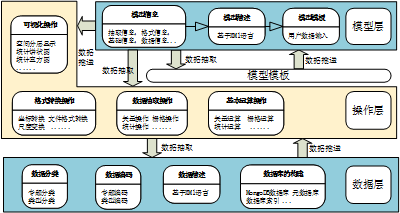
\includegraphics[angle=0,width=10cm,height=7cm]{pic/road.png}
\caption{技术路线}
\label{fig:1}
\end{center}
\end{figure}
%------

\subsection{论文结构}
本文总共分为五章:

第一章:绪论,主要是介绍本文的主要研究的背景,现在国内外关于相关技术的研究现状和论文的主要研究技术路线。

第二章:多源地理数据的分类与数据库的构建,主要是通过学习,总结现有的地学数据分类方法,构建本文的基于专题和数据类型的地理数据分类方法。同时引入非关系型数据库-MongoDB来建立多源地理数据的数据库。

第三章:地理模型数据需求引导的数据抽取与推送,通过分析地理模型,了解地理模型对数据的详细需求,以此建立地理模型数据需求模板。结合常用地理数据操作函数和多源地理数据分类体系,建立数据操作流模板。综合地理模板,操作模板和多源数据库,架构针对地理模型的数据抽取与推送数据流。

第四章:系统实现与案例,利用以上思路,搭建原型系统,并结合江苏沿海滩涂健康评价模型,验证思路的正确性。


\chapter{多源地理数据的分类与数据库的构建}
\section{多源地理数据的分类与描述}
地理数据分类,与地理数据编码,是地理数据库建库之前就需要解决的问题。数据分类是数据编码的基础,为GIS的应用与推广,起到了基础性的作用。由于地理学涵盖内容非常的广,包含的专题非常多,同时地理数据的获取方法日新月异,数据格式多种多样,又缺乏相对统一的地理数据分类体系,也就导致许多地理数据在不同的分类体系中重复出现。这极大的阻碍了地理数据的共享和有效利用。为了保证地理数据与地学模型之间的准确匹配,有必要解决多源地理数据的分类体系问题,同时也使得地理数据 的科研,管理等向标准化,规范化方向发展。本文基于国家科学数据分类规范,基础科学数据分类规范和专题地图信息分类与代码的基础上,结合地理模型的数据需求,构建了多源地理数据的分类体系和编码,并采用半结构化的XML Schema对数据进行了描述。

\subsection{多源地理数据的产生与表现}
多源地学数据的产生与表现主要可以概括为以下四个方面:语义多样性,时空和尺度多样性和获取手段多元性,数据格式的多样性。

1. 语义多样性:由于地理信息系统的多样性研究对象,决定了地理数据具有多语义
性的特点。在现实世界中,几何特性一致的地理数据单元,在不同的场合却可以表示为不同的含义,比如:一个数据可以表示地理位置,海拔高度,气候,地貌,土壤等自然地理特征,同时也可以表示经济社会信息,如行政区编号,人口数,GDP 等。同时针对解决的问题不同,地理数据的也存在语义的分异问题。

2. 时空和尺度多样性:时空性和尺度性是地理数据有别于其他科学数据的重要方面。一个地理信息系统中的数据即可以表示:相同时间情况下的不同地理空间数据 ,也可以表示在相同的地理空间条件下的不同时间产生的数据。另外,即使在相同时间,相同地理空间下的数据,在不同尺度下的研究也具有不同的意义。

3. 获取手段多元性:随着技术的发展,地理数据的获取手段越来越多,设备越来越先进,主要地理数据获取设备包括:图标,统计报表,现场测绘,航空航天测量,激光雷达,GPS,等。这些不同手段获取来的数据,通常具有不同存储格式,不同的应用场景,提取和处理手段也不尽相同。

4. 数据格式的多样性:地理数据包括:空间数据和属性数据,使地理数据不仅包含空间的存储格式,又有属性的存储格式。同时不同系统又有各自系统支持的不同数据格式。【】

\subsection{多源地理数据的分类原则}
由于地理数据的复杂性特点,所以地理数据的分类不是简单的归并和聚类,需要确定数据的类别,以达到对该类数据或其子数据分类的结果在意义上的无歧义性。数据分类的好坏,直接影响到数据的应用,组织,生产和共享,更可能导致重复的投入与建设,同时,为了促使分类结果的一致性认可,必须基于一定的既定标准和准则。本文在指定分类系统时,尽量保持与国家基础科学数据分类的一致性,同时针对自身地学地理模型的数据需求,进行实用性扩展。

1)	尽量采用已有的国家标准
在编制本文的分类系统过程中,主要借鉴科学数据分类规范与分类词表,基础科学数据分类规范和专题地图信息分类代码等分类方法

2)	保证分类的系统性与完备性

数据分类体系需要保证一定的包容性和概括性,要能够同时兼容现有的地理数据,又同时能够包容将来可能产生的数据类型。分类的结果能够让数据的本身和数据的属性之间保持一定的完整性,使得每一个数据都能找到其对应的分类位置;

3)	层次性原则

多源地理数据的划分,同其他数据、其他分类体系一样,应该具有层次性,采用自上而下,或者自下而上的划分方法。保证数据划分结果的结构明晰性;

4)	实用性原则

分类方法既要考虑数据在大范围上的包容性,又要考虑数据组织,存储与管理,同时还需要注意用户的查询,检索时候的习惯性;

5)	模型的适应性

数据只有通过模型才能更好的转化为信息,多源地学数据在分类的时候也应该充分考虑模型的适应性,方便模型的对数据的无二义性和准确性获取和使用。

\subsection{多源地理数据分类体系}
本文采用线分类法,将多源地理数据划分为两层,分别是:专题数据层和数据类别层。
将地理专题数据划分为四个层次。主题层,第一层,第二层和具体层,主要是从地理信息专题属性出发,确定数据在高层次上的类属性,是主要的数据分类层。采用自上而下的分类,分别为:主题层表示专题名称,第一层和第二层表示专题的子类,具体层则表示具体数据。

数据类别层划分为三层,数据类型层,数据维度层和数据尺度层。主要是从具体的数据类型出发,为方便数据的统一存储,组织,管理和模型的数据匹配出发的。数据类型层主要表示数据所属的类别。

根据上述的原则与方法,结合现有的多源地学数据资源的实际情况。本文的多源地学数据的分类体系一般描述如下:$M_0 = {m_{i,j} \in m_i | R _{i,j}} i = 1,2,\cdots n, j = 1,2,\cdots m$ 式中$R_{i,j}$为第 $i$类数据的分类体系;$m_{i,j}$为第$i$类数据的第$j$个具体类型。本文形成了多源数据资源分类体系(见表)

% Booktabs require to add \usepackage{booktabs} to your document preamble
\begin{table}[t]
\caption{数据专题分类}\label{tab:table2.1}
\begin{center}
\begin{tabular}{@{}lll@{}}
\toprule
主题层   & 专题层 & 子类层                    \\ \midrule
基础数据层 & 水系  & 河流、运河、水库、沼泽、海域...      \\
      & 交通  & 铁路、公路、航空...            \\
      & 行政区 & 国家级、省级、市级、县级...        \\
      & ...    & ...                       \\
专题数据  & 地质  & 普通地质、工程地质、水文地质...      \\
      & 气候  & 气候区划、气候类型...           \\
      & 人口  & 性别构成、年龄构成、职业构成、文化程度... \\
      & 经济  & 工业、农业、服务业、GDP、财政收入...  \\
      & 环境  & 空气污染、水体污染、土壤污染...      \\
      & ...    &  ...                      \\ \bottomrule
\end{tabular}
\end{center}
\end{table}

\newcommand{\tabincell}[2]{\begin{tabular}{@{}#1@{}}#2\end{tabular}}
  
\begin{table}[!htp]           %存在问题:下一行要左对齐
\caption{数据类型分类}\label{tab:table2.2}
\begin{center}
\begin{tabular}{llll}
\hline
 数据类型    &  文件后缀名                  &  维数                                              &  数据描述                                                          \\ \hline
 矢量数据    &  Shapefile;Mif;DXF;E00;  &  2维                                               &  在矢量数据中,用点、线、面表达现实世界。                          \\
 栅格数据    &  DEM;ASCII;SRTM;          &  2维                                               &  \tabincell{c}{在栅格模型中,用空间单元(Cell)或像元\\(Pixel)来表达现实世界;}   \\
 场数据      &  NetCDF;                    &  n维                                               &   \tabincell{c}{连续场将真实世界描述为有限变量,每个变\\量定义在任何可能的位置上;}  \\
 点云数据    &  Asc;Txt                    &  3维                                               &  点云数据具有几何位置和强度信息;                                  \\
 二维表      &  Excel;table;  Txt;Cxv;  &  2维                                                & \tabincell{c}{ 二维表由行列组成,以行号列号唯一确定表\\中的数据;}\\
 时间序列    &  XML;Txt                    &  1维                                               &  对同一对象不同时间连续观察所取得的数据;                          \\
 文本数据    &  Txt;                       &  1维                                               &  用文本来存储的数据形式;                                          \\
 数值数据    &  Txt;                       &  1维                                               &  用变量来表示数值的存储形式;                                      \\  \hline
\end{tabular}
\end{center}
\end{table}

\subsection{多源数据的分类编码}
数据的编码是将分类好的数据结果,用一种方便计算机和人识别的符号系统来表达出来的过程,编码的结果是代码,由数字或字母组成。根据专题地图信息分类与代码的等长性,唯一性,可扩充性,合理性,简单性,实用性和规范性等信息编码原则,本文构建了如图  所示的数据专题分类编码和数据类型分类编码。

\textbf{两个图}

本文以基础科学数据分类规范为专题数据基础,采用第一位为主码,0表示数据是基础地理数据,1表示专题数据 。后两位分别表示数据所属的专题和具体的数据描述(如:人口年龄、人口密度等 )。

对于数据类型分类,本文借鉴美国地质调查局(USGS)制定的《数字线划图形标准》采用五位数字的代码结构,将前三位设为主码,后两位为子码。主码的前二位数字用以惟一定义要素的类别,主码的第三位数宇是子码的解释位:如果为零,表示子码是要素的分类码;如果非零,表示子码是要素的参数值或称为参数属性代码,例如地形高程、河流长度等等。子码的第一位数字表示数据的维度(1维,2维,3维),第二位数字标识数据要素的表现尺度(国家级,省级,县级等)。因此,该编码系统具有分类逻辑性强,代码信息量丰富,便于进行要素间关系的推理判别等特点。

\section{多源地理数据的描述方法}
\subsection{XML Schema语言介绍}
XML(Extensible markup language) 意为可扩展标记语言,是 world wide web 发展的一个重要里程碑,而且成为了 web 上数据交换和表示的标准。它使用有意义的标记(TAG)来识别数据,并且可以按照用户的需求来增加标记,如数学标记语言 MATHML,电子商务标记语言 EBXML,地理标记语言 GML 等。半结构化的 XML 具有半结构化模式的基本特点,第一,先有数据,后又模式,这跟 NoSQL 的设计风格非常相似,使得它具有非常好的数据包容性。第二,动态变化,数据和模型通常处于不断的更新之中,而半结构化的模式使得在不改变原来结构的基础上保持动态的变化。

采用什么元素、标记、属性和实体,是解决多源地理数据XML描述首先要知道的;因此,如何反映这些描述信息之间的逻辑关系,即定定一个地理元数据的XML描述模式。通常有两种做法,第一是DTD(XML文档类型定义)和XML Schema。

XML Schema是用于描述和规范XML文档的逻辑结构的一种语言,与DTD相较而言,XML Schema具有一下五个优势:

    1.一致性

    与DTD不同,XML Schema不是同EBNF语法,而是直接借助XML本身的特性,用XML语法来定义文档的模式,使得XML文档及其模式定义实现了从内到外的统一。此外,XML Schema本身是一种XML文档,可以被现有的XML编辑制作工具所编辑,被XML语法解析器所解析,被XML应用系统所利用,使现有的XML文档得到了最大程度的保护。

    2.扩展性

    尽管DTD中定义了一些数据类型,但基本都是针对属性类型定义的,并且类型非常有限。XML Schema不仅支持DTD中的所有原有数据类型(诸如标识和标识引用之类的类型),还支持整数、浮点数、日期、时间、字符串、URL和其它对数据处理和验证有用的数据类型。除了规范中定义的数据类型以外,还可以利用XML Schema创建自己的数据类型,并且可以基于其他数据类型那个派生出新的数据类型类型,具有良好的可扩展性。

    3.易用性

    作为一种XML API,DOM和SAX只是对XML实例文档有效,对于DTD则无能为力,不可能通过DOM或SAX来判断在DTD中一个元素的属性类型或者某个元素的子元素允许出现的次数。但是,使用XML Schema则不存在这一问题,因为对XML文档结构进行描述的XML Schema是一种“形式良好的”XML文档,用DOM和SAM去访问和处理就非常容易了。

    4.规范性

    XML Schema同DTD一样,提供了一套完整约束机制来规范XML文档中元素的使用,但相比之下,XML Schema基于XML语法,更具规范性。XML Schema利用元素的内容和属性来定义XML文档的整体结构,如哪些元素可以出现在设计的文档中,元素间的关系是什么、每个元素有哪些内容和属性以及元素出现的循序和次数等,都一目了然。

    5.互换性

    正如每个人都可定义自己的DTD一样,当然也可以设计适合自己需求应用的XML Schema,并且可以同其他人交换自己的XML Schema。另外,也可以通过映射机制,将不同的XML Schema进行转换,以实现更高层次的数据交换。


\subsection{基于Schema的地理元数据描述}
地理元数据是地理信息中用于描述地理数据集的内容、质量、表示方式、空间参考、管理方式以及数据集的其他特征,它是实现地理空间信息共享的核心标准之一。
它统一了对地理数据元数据的理解和认识,
帮助数据使用了解数据的相关信息,比如:数据的格式,发布单位,空间分辨率等;
用来建立地理数据目录和数据交换中心,通过数据目录和数据交换中心等提供的空间元数据内容,用户可以共享空间信息、维护数据结果,以及对它们进行优化等;
提供数据转换方面的信息。使用户在获取空间信息的同时便可以得到空间元数据信息。通过空间元数据,人们可以接受并理解空间信息,与自己的空间信息集成在一起,进行不同方面的科学分析和决策。描述空间信息的元数据标准体系内容按照部分、复合元素和数据元素来组织,它们是依次包含关系等;提供了数据操作库接口设计标准,通过元数据,可以实现多源数据与操作函数这间的对接。

地理元数据包含的内容较多,主要有:数据的内容信息,数据的参考信息,数据的基础信息,数据的应用信息等。本文主要通过地理元数据实现对模型的匹配和对数据操作接口的匹配。所以本文的数据元数据包括了数据的基本信息和关键的数据编码信息,数据类型,空间,尺度等信息。

本文研究内容的地理元数据主要内容如下所示:

\textbf{元数据结构图}

本文基于XML Schema的地理元数据描述如下所示:
\textbf{XML Schema 地理元数据}



\section{多源地理数据库的建立}
\subsection{非关系型数据库介绍}
NoSQL(not only SQL)即“不仅仅是SQL”,指的是非关系型数据库,是一项全新的数据库革命性的运动。NOSQL作为新兴数据库系统概念,由于其少量数据处理能力,近年来备受各大IT公司的欢迎。Google的Bigtable,Facebook的Cassandra,Apacha的Lucene,等等。起来越多的受到人们的重视。

NoSQL和所有其他事务一样,它的兴起也是由很多理论支撑作为前提的,正是由于下面的一些理论支撑,NoSQL的发展才如此的明朗。
\begin{itemize}
\item{CAP理论}

CAP(Consistency,Availability,Patition tolerance)理论论述的是,在任何分布式系统中,只可能满足一致性,可用性以及分区容忍性三者中的两个,不可能全都满足。
\item 一致性Hash

一致性Hash主要是为了解决P2P环境中最为关键的问题:如何在动态网络拓扑中存储和路由。当一个节点失效的时候,其他节点的数据不会受到失效节点的影响,而这个节点的数据会被分流到另外的一个节点。而增加一个节点时,只会对一个节点的一部分数据有影响。
\item Gossip

Gossip是一个应用于P2P中的协议,它主要是通过一个N节点集群中的每一个节点与所有其他N-1个节点进行通信,实现数据同步。

\item 易扩展性

非关系型数据库,数据这间的无关性,让NoSQL具有了非常好的扩展性,也让数据库在架构的层面上带来了可扩展的能力。
\item 灵活的数据模型

这个特性让NoSQL能够轻松的应对结构化,半结构化和非结构化的数据
\item 大数据量,高性能

NoSQL数据库通常具有非常好的读写性能,尤其是在大数据量上。这依旧得益于它的数据无关性,数据库的结构简单性。
\end{itemize}

\subsection{NoSQL的分类}
NoSQL数据库种类很多, 划分的方式也很多,现在主要是从数据库的存储模型上来分,主要可以划分为列式存储,文档存储,Key-Vlaue存储,图存储,对象存储和XML数据库等。具体的分类方法如下表如示:

\begin{table}[!htp]           %存在问题:下一行要左对齐
\caption{NoSQL数据库分类}\label{tab:NoSQL_class}
\begin{center}
\begin{tabular}{lll}
\hline
 类型           &  部分代表       &  特点                                \\
\hline
 列式存储       &  Hbase          &  该类数据库是按列存储数据的,最大        \\
                &  Cassandra      &  特点是方便存储结构化和半结构化的        \\
                &  Hypertable     & 数据,方便做数据压缩针对某一列或      \\
                &                 &  者某激烈的查询有非常大的IO优势。    \\
 文档存储       &  MongoDB        &  文档存储一般用类似json的格式存储,  \\
                &  CouchDB        &  存储的内容是文档形式的,这样也就    \\
                &                 &  有机会对某些字段建立索引,实现      \\
                &                 &  关系型数据库的某些功能              \\
 Key-value存储  &  Tokyo Cabinet  &  该类数据库可以通过Key快速查询到     \\
                &  Berkeley DB    &  value,一般来说,存储不管value的    \\
                &  MencacheDB     &  格式,容纳性很强                    \\
 图存储         &  Neo4j          &  图形关系的最佳存储,使用传统关系    \\
                &  FlockDB        &  数据库来解决的话性能低。            \\
 对象存储       &  db4o           &  通过类似面向对象语言的语法操作数  \\
                &  Versant        &  据库,通过对象的方式存储数据          \\
 xml数据库      &  BerkeleyDBXML  &  高效的存储XML数据,并支持XML  \\
                &  BaseX          &  的内部查询语法,比如:XQuery          \\
 \hline
\end{tabular}
\end{center}
\end{table}

\subsection{MongoDB数据库介绍}
MongoDB数据库是一个介于关系数据库和非关系型数据库这间的产品,是非关系数据库当中功能最丰富,最低关系数据库的。它支持的数据结构非常松散,是类似json的Bson格式,因此可以存储枈复杂的数据类型。MongoDB最大的特点是它支持的查询语言非常强大,其语法有点类似于面向对象的查询语言,几乎可以实现关系型数据库单表查询的绝大功能。,而且还支持对数据建立索引。下图主要表现MongoDB数据库和常规关系型数据库存储模式的比较:


%------
\begin{figure}[!htb]
\begin{center}
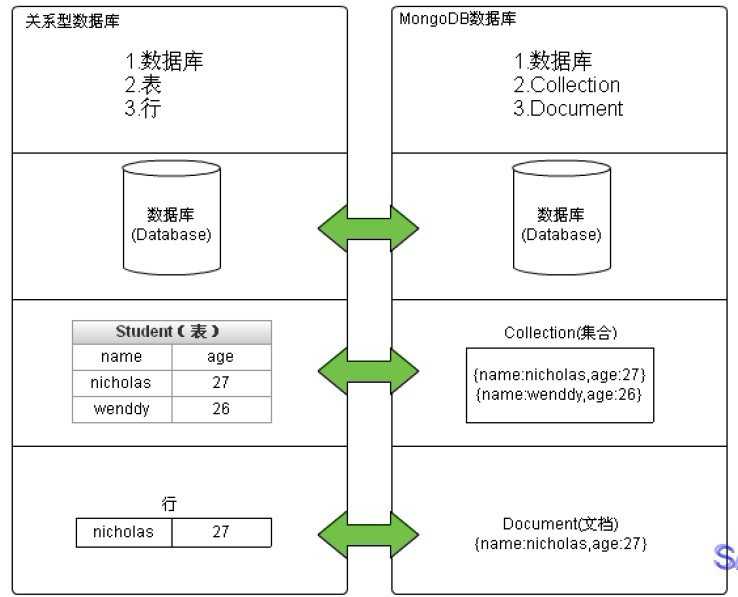
\includegraphics[angle=0,width=1\textwidth]{pic//mongoDB_fileType.jpg}
\caption{MongoDB的文档结构}
\label{fig:1}
\end{center}
\end{figure}
%------

MongoDB主要解决的是海量数据的访问效率问题,根据官方的文档,当数据量达到50GB以上的时候,Mongo的数据访问速度是MySQL的10倍以上。Mongo主要是支持海量,非结构化的数据存储的,它还自带了一个出色的分布式文件存储系统-GridFS,可以支持海量数据的存储。同时因为Mongo的松散文档存储模式,可以支持复杂的数据结构如shapefile,而且带有强大的数据查询功能。

\begin{itemize}
\item 丰富的数据模型:
MongoDB是面向文档的数据库,将关系数据库中“行”的概念换成了更加灵活的“文档”(document)模型。面向文档的方式可以记录和表示非常复杂层次关系。MongoDB是没有模式的,文档的键(key)不需要事先设定,开发者可以非常容易的变更数据模型。
\item 易扩展性:
MongoDB利用其面向文档的数据模型,使其可以自动在多台服务器之间分割数据,还可以平衡集群之间的数据和负载,自动重排文档,这样开发者只需要专注于编写应用程序,而不是考虑如何扩展。
\item 功能丰富:
索引功能,mongodb具备通用的辅助索引,同时也提供唯一的,复合的, 地理空间索引能力。
\item 存储和查询支持javascript:
开发人员可以直接在服务端存取javascript的函数和值,
\item 聚合:
MongoDB支持MapReduce和其他聚合工具,等等功能
\item 简单的管理与维护:
Mongodb尽量让服务器自治的简化数据库的管理,如果主服务器挂掉,Mongodb会自动切换到备份服务器上,并将备份服务器升级为活跃服务器。
\item 多语言的支持:
支持RUBY,PYTHON,JAVA,C++,PHP,C\#等多种语言。
\item 拥有GridFS存储结构:
MongoDB使用高效的二进制数据存储,包括大型对象(如视频等)。
\end{itemize}

\subsection{基于MongoDB的地学数据存储}
 MongoDB在执行数据插入的时候,使用驱动程序讲数据转换为BSON的形式,然后将其送入到指定的数据库当中。数据库解析BSON格式的数据,检验是否包含"\_$id$",
除此之外不做别的数据验证,这样不仅提高的插入的效率,也提高了数据的安全性,远离了数据库的注入式攻击。减少了关系型数据库的完整性验证,可靠性验证等复杂的数据 有效性检查(文档是否超长,是否包含UTF-8字符,是否格式不对等等)的时间和繁琐。

    mongodb将数据插入到数据库的集合中,主要使用: MongoDB 的  insert() 或 save() 方法。mongodb在插入数据的时候,并不需要事先创建数据库和集合,数据库和集合都是在第一次插入文档的时候才会被创建。
这个行为与mongodb对数据的动态处理方式是一致的,因为不用事先定义文档的结构,单独的集合和数据库可以在运行时才被创建。这样的方式能够简化并加速开发的过程,而且有利于动态分配命名空间。

\subsubsection{MongoDB存储空间矢量数据}
地学空间数据具有数据种类多,数据量大,数据来源丰富,数据结构复杂等特点,所以对地学数据的存储要求也非常的高。对地学数据的存储,通常有以下几个要求:
\begin{itemize}
\item 存储和管理海量空间数据的能力。随着地学数据获取手段的不断增加,技术的不断革新,地学空间数据的增长,正呈现几何级数的增长中。存储和管理海量地学空间数据就成为选择数据库的基础条件。而MongoDB作为NoSQL数据库中的一员,也具备了这种能力。

\item 快速的数据传输,处理能力。现在的地学应用越来越向网络方向发展,地学数据的传输,处理,高并发性等问题都将是未来或者现在正面临的问题。而MongoDB作为为网络应用而生的数据库,能够更好的面向未来的发展。

\item 良好的数据安全性。地学数据分析常常具有不可复原的特点,这就要求数据库必须具有良好的备份机制。MongoDB 采用冗余,增量,日志多种备份方式,能够最大限度的保证数据的安全性。
\end{itemize}

  本文以shapefile空间数据为例,利用开源库GDAL读取shapefile将其插入到MongoDB数据库中。程序读取shapefile 中的每一条数据,并将其保存为字典形式,利用MongoDB数据库的Insert方法,将获取的Shapefile数据导入数据库中。相对于关系型数据库要简单得多;shapefile数据入库代码如下所示:
\begin{verbatim}
#+Name:<shapefile into MongoDB>
#-------------------------------------------------------------------
: def  insertShp2mongo(self, ds, shp_db, shp_collect, meta_db, 
;				meta_collect, meta_data):
:     lyr = ds.GetLayer()
:     feat = lyr.GetNextFeature()
:     totfeats = lyr.GetFeatureCount()
:     meta_data = self.get_metedata(ds)
:     mongo_bll.insert(meta_db, meta_collect, meta_data)
:     while feat:
:         mongofeat = {}
:         geom_data = self.getOneGeomData(feat)
:         feat_defn = lyr.GetLayerDefn()
:         attri_data = self.getOneAttributeData(feat, feat_defn)
:         mongofeat = dict(geom_data , **attri_data)
:         mongo_bll.insert(shp_db, shp_collect, mongofeat)
:         feat.Destroy()
:         feat = lyr.GetNextFeature()
#+END_SRC
\end{verbatim}

 MongoDB的每一个数据库都有自己独立的文件。如果开启了directoryperdb选项,则会为每一个数据库建立一个单独的文件夹。
  数据库文件在内部会被切分成单个的块,每个块只保存一个名字空间的数据。在MongoDB中,名字空间用于区分不同的存储类别。比如每个collection有一个独立的名字空间,每个索引也有自己的名字空间。
  在一个块中,会保存多条记录,每条记录是BSON格式,记录与记录之间通过双向链表进行连接。
  一个shapefile文件存储在一个collection当中。shapefile在MongoDB中的存储表现如下:

\begin{verbatim}
#+Name:<shapefile in MongoDB>
: {
:     "_id" : ObjectId("4dc82e7f7de36a5ceb000000"),
:     "PERIMETER" : 0,
:     "NAME" : "漠河县",
:     "PYNAME" : "Mohe Xian",
:     "AREA" : 0,
:     "ADCODE93" : 232723,
:     "CNTYPT_ID" : 31,
:     "CNTYPT_" : 1,
:     "geom" : {
:         "type" : "Point",
:         "coordinates" : [
:             122.53233,
:             52.968872
:         ]
:     },
:     "ID" : 1031,
:     "PN" : 1,
:     "CLASS" : "AI"
: }
#+END_SRC
\end{verbatim}

上面是shapefile数据中的一个document,使用的是BSON数据格式,数据的结构一目了然。其中的''geom''即为Geometry类型的数据,即地理空间数据,也是采用BSON格式存储,这样的存储格式为后续的空间索引与空间查询带来便利。

MongoDB原生地支持了空间索引与空间查询,这一点比PostgreSQL和其他关系型数据库更方便,不再需要再进行空间扩展了。而在关系型数据库中,不能够直接实现shapefile数据库的存储,虽然现在SQL server,Oracle等都开始对空间数据提供支持,但是仅仅体现在对空间数据的识别和可视化基础上,依然不能实现对shapefile等数据的直接存储,因为关系型数据库的强关联性,对非结构化的空间数据支持不够好,需要通过第三方软件的转换才能够存储到数据库中。

MongoDB与SQL server数据库存储shapefile数据的效率的对比
%------
\begin{figure}[!htb]
\begin{center}
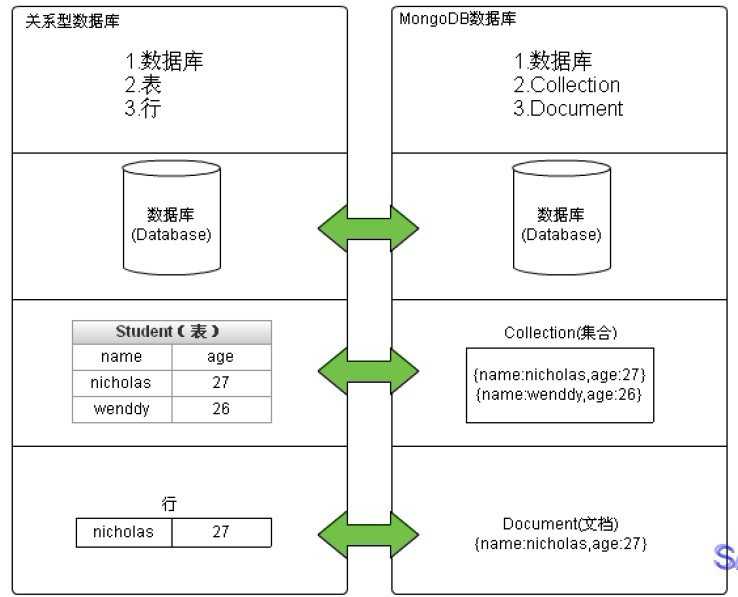
\includegraphics[angle=0,width=1\textwidth]{pic//mongoDB_fileType.jpg}
\caption{MongoDB的文档结构}
\label{fig:1}
\end{center}
\end{figure}
%------

\subsubsection{MongoDB存储空间栅格数据}
 GridFS是一种在MongoDB中存储大二进制文件的机制,使用GridFS存储文件有如下几个原因:
\begin{enumerate}
\item 可以利用GridFS简化需求,不需要使用独立的文件存储架构
\item GridFS会直接利用业已建立的复制或者分片机制,所以对于文件存储来说故障恢复和扩展都很容易
\item GridFS可以避免用于存储用户上传内容的文件系统出现的某些原因,例如:GridFS在同一个目录下放置大量的文件是没有任何问题的。
\item GridFS不产生磁盘碎片,因为MongoDB分配数据文件空间的时候,是以2GB为一块的。

\end{enumerate}
    针对栅格数据的特点,和MongoDB单条数据不超过16M的要求,本文主要借用【】的方法,采用地图瓦片数据存储方案。首先对原始图像进行坐标转换与地图配准。设定每张瓦片的大小为256*256。以后不同等级(即分辨率)的地图之间采用四叉树分图。
例如第一层上的瓦片四叉树化后到第二层则裂变为4张,分别以四个象限作为编码方案,即第一象限(1),第二象限(2),第三象限(3),第四象限(4)
每一子块的编码等于所属的父块编码再加上自身编码的组合。如图所示:

%------
\begin{figure}[!htb]
\begin{center}
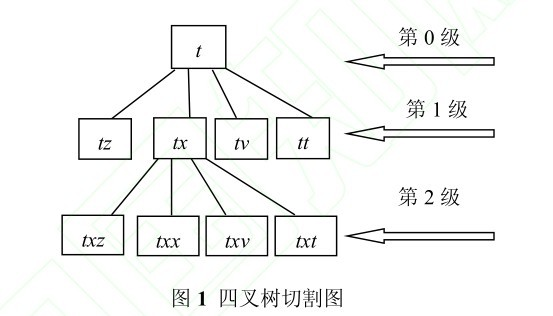
\includegraphics[angle=0,width=10cm,height=7cm]{pic//sichashu.jpg}
\caption{栅格地图四叉树切割}
\label{fig:2}
\end{center}
\end{figure}
%------

当需要查找,或者显示某块地图时,根据如下公式可以计算得出地理坐标与图片编码之间的关系,即可以得出所需要显示的栅格图片。
第L层第I行,第j列位置切片的地理坐标范围计算公式如下:
\begin{itemize}
\item $ curXMin = XMin + j*(\Delta\{x\}/m*2^{L-1})$
\item $ curXMax = XMin + (j+1)*(\Delta\{x\}/m*2^{L-1})$
\item $ curYMin = YMax - (i+1)*(\Delta\{y\}/n*2^{L-1})$
\item $ curYMax = YMAX - i*(\Delta\{y\}/n*2^{L-1})$
\end{itemize}
反算瓦片行列号的公式如下:
\begin{itemize}
\item $i = \max{[(YMax -y)/\Delta{y}]*n*2^{L-1}}$
\item $j = \max{[(x-XMin)/\Delta{x}]*m*2^{L-1}}$
\end{itemize}
其中,XMin,XMax表示地图的最大,最小经度值,YMin,YMax表示瓦片地图的最大最小维度值;
$\Delta\{x\}$表示地图的横坐标差,$\Delta\{y\}$表示地图的纵坐标差,即地图分辨率。
$m*2^{L-1}$,$n*2^{L-1}$分别表示第L层瓦片地图的行列数目。基于Python的MongoDB瓦片存储的代码如下:
\begin{verbatim}
#+Name:<raster into MongoDB>
#+BEGIN_SRC<Python><swithces><header arguments>
,Connect = mongo.connect("localhost",27017)
,db      = Connect.getDB("ImageFS")
,collect = db.getCollection("imageCollect")
,....
,data = {}
,data["map_id"] = getCutImageData(image_file_path)
,data["size"]   = fileSize
,collect.insert(data)    #插入到数据库中
#+END_SRC
\end{verbatim}

为了验证基于MongoDB的瓦片存储策略,我们搭建了如下的系统环境:

一台CPU为Intel(R)Core(TM)i5-2400 3.10GHz,内存为2GB,操作系统为Windows XP 64位操作系统上进行存储实验。
分别利用MongoDB 2.40,和SQL Server 2008存储对比。将预先生成的十二层数据,第L层有$2^{L-1}*2^{L-1}$张图片,平均每张大小为25kb,实验取预生成的第8层,10层,12层数据为案例,三层的数据量大小分别为:180M,860M,5.5GB,得到存储时间对比:

%------
\begin{figure}[h]
\begin{center}
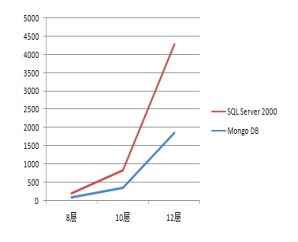
\includegraphics[angle=0,width=10cm,height=7cm]{pic//raster_insert.jpg}
\caption{栅格数据存储时间对比}
\label{fig:3}
\end{center}
\end{figure}
%------

上图可以看出,随着数据量的不断增大,MongDB和SQL Server的插入时间都出现大幅度的增长,但是到第12层的时候,
两者之间的差距就达到了2.3倍,可以体现出MongoDB在存储大数据文件上的高效性。

\subsubsection{MongoDB存储地学统计数据}
MongoDB自带的数据导入工具mongoimport可以把一个特定格式文件中的内容导入到指定的collection中,该工具可以导入JSON格式数据和csv格式数据。但是该工具对格式的限制使很多其他格式的统计文档很难实现导入。
所以通过把地学统计数据转换为字典格式,可以支持更多的文件格式,可控性也更强。
下面是利用Python代码将excel数据转换为dict格式 ,然后insert到MongoDB中。

\begin{verbatim}
#+Name:<raster into MongoDB>
,def insertExcel2Mongo(self, db):
,    sheetNum = getSheetNum() #获取excel中sheet数目
,    collet   = getCollection(database) #获取集合
,    while i<sheetNum:
,       sheetName = getSheetNameByIndex(i) #获取sheet名字
,       sheetData = getSheetData(i)        #获取sheet数据
,       collect.insert(sheetData)          #插入到MongoDB
#+END_SRC
\end{verbatim}

%------
\begin{figure}[h]
\begin{center}
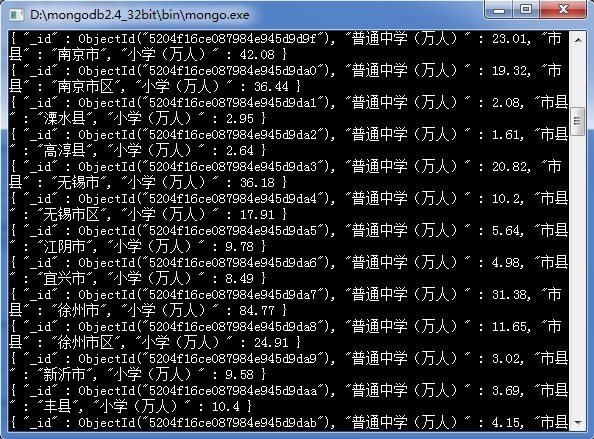
\includegraphics[angle=0,width=10cm,height=7cm]{pic//excel_data.jpg}
\caption{MongoDB中统计数据集合文档内容}
\label{fig:4}
\end{center}
\end{figure}
%------
利用同样的环境,分别将10万条,100万条,1000万条数据插入到MongoDB和SQL Sever中,进行存储效率的对比。
得到的存储时间对比结果如下图所示:

\subsection{基于MongoDB的地学数据查询}

\subsubsection{MongoDB数据检索}
MongoDB查询数据主要是利用find()函数和查询文档对数据库执行查询。它使用''\$''条件查询实现范围,集合包含、不等式、和其他查询。 
对于复杂的查询,MongoDB可以使用$where$子句和强大的Javascript来表达。
  MongoDB查询的结果返回一个数据库游标,MongoDB游标只有在你需要的时候才会惰性的批量返回文档。
  find()函数的基本形式是:find(\{\},\{\}),第一个参数决定需要返回哪些文档,第二个参数则是在不需要将文档所有键/值对都返回的时候,通过它来指定想要的键。
  MongoDB的查询还能够通过添加查询条件来提供更加复杂的查询。
find函数还可以通过添加查询条件,perl兼容的正则表达式,支持Javascript语言的where查询等,来提供复杂的查询要求。
下图展示了MySQL同MongoDB查询语句之间的联系和区别:

%------
\begin{figure}[!htb]
\begin{center}
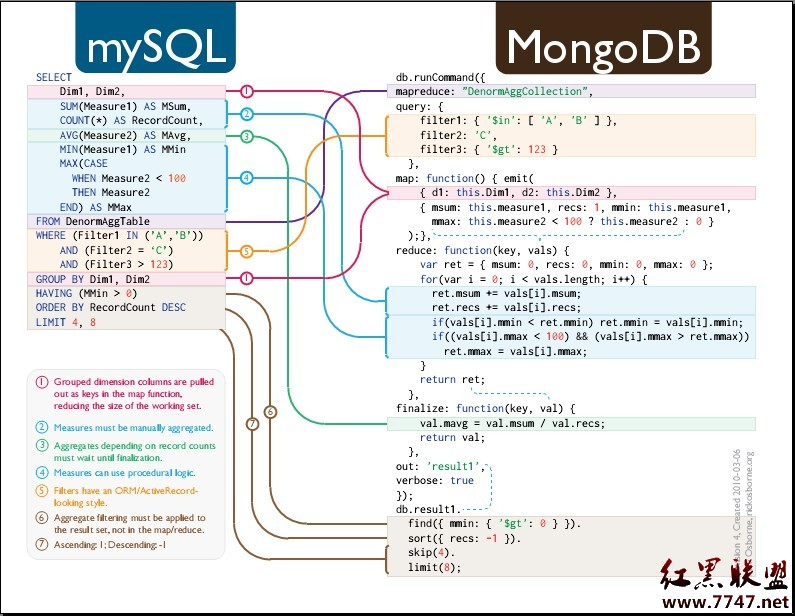
\includegraphics[angle=0,width=10cm,height=7cm]{pic//mongodb_Mysql.jpg}
\caption{MongoDB与MySQL查询语句对比}
\label{fig:5}
\end{center}
\end{figure}
%------

MongoDB空间索引
Mongodb内部使用B树来表示索引。B树有两个显著的特点,第一,它们能用于多种查询,包括精确匹配,范围条件,排序,前缀匹配和仅用索引的查询。
第二,在添加和删除键的时候,他们能够依然保持平衡,这两个特点让b树成为了数据库索引的理想选择。下图是MongoDB 中B树索引的示例:

MongoDB同时为坐标平面查询提供了专门的索引:地理空间索引。这也是全球流行的LBS服务foursquare选择MongoDB的原因之一。MongoDB通过B+Tree数据索引结构实现地理空间索引。
地理空间索引实现原理如下图所示:

\begin{figure}[h]
\centering
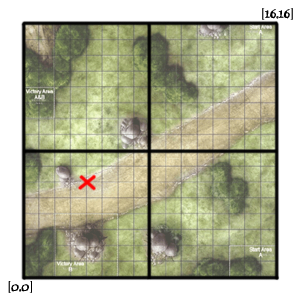
\includegraphics[angle=0,width=6cm]{pic//map2.png}
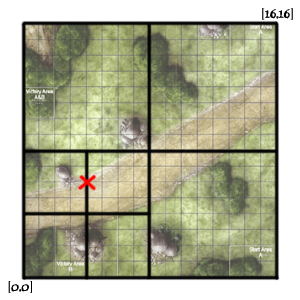
\includegraphics[angle=0,width=6cm]{pic//map3.png}
\caption{第一和第二步}
\end{figure}

\begin{figure}[h]
\centering
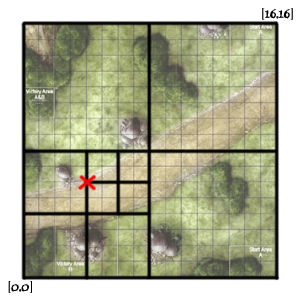
\includegraphics[angle=0,width=6cm]{pic//map4.png}
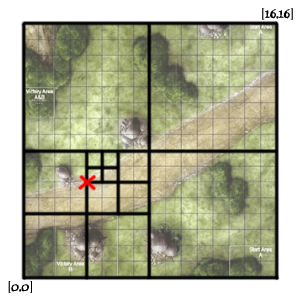
\includegraphics[angle=0,width=6cm]{pic//map5.png}
\caption{第三和第四步}
\end{figure}

单纯的[x,y]数据是无法建立索引的,所以MongoDB在建立索引的时候,会根据相应字段的坐标计算一个可以用来用作索引的hash值,这个值叫做geohash。
图中以地图上坐标为[4,6]的点为例,第一步将原始图划分为等大小的四块,分别为:左下00,左上01,右下10,右上11.

\begin{center}
\begin{tabular}{|r|r|}
\hline
 01  &  11  \\
\hline
 00  &  10  \\
 \hline
\end{tabular}
\label{table:1}
\end{center}

则得到目标点的geohash值为00.继续划分,第二步得到目标点的geohash值为0011,依次类推,最终得到目标点的geohash 值为:00110100。这样我们用这个值来做索引,则地图上点相近的点就可以转化成有相同前缀的geohash值了。

\subsubsection{MongoDB的空间数据查询}
假设,要找到给定经纬度坐标周围的最近的其他对象,就需要创建一个专门的索引来提高类似的查询效率,MongoDB 支持二维空间索引,所以在进行空间数据查询前,必须对空间数据进行索引构建。mongodb中建立二维地理位置索引的命令如下:

\noindent >db.xpoint.ensureIndex(\{'geom.coordinates'':''2d''\})

如此,便建立了集合xpoint的二维空间索引。
执行空间数据库查询命令\$near,\$within, \$circle,\$polygon\ldots{}.

执行空间数据查询的时候,geom.coordinates键值必须是某种形式的一对值:一个包含两个元素的的数组,或是两个键的内嵌文档。如下所示:

\noindent \{''geom.coordinates'':[1,100]\}\\
\{''geom.coordinates'':\{''x'':30,''y'':20\}\}\\
\{''geom.coordinates'':\{''latitude'':29,''longtitude'':123\}\}

默认情况下,地理空间索引假设值的范围是[-180,180],要是想用其他值,可以通过ensureIndex的选项来指定最大,最小值:

\noindent > db.xpoint.ensureIndex(\{''geom.coordinates'':''2d''\},\{''min'':-50,''max'':50\})

地理空间查询以两种方式进行,第一,普通查询,即精确点位查询方式,实际用途不多。
第二,目标点的临域查询(\$near),和范围查询(\$within)。
临域查询的结果是按照目标点由远及近的方式,将集合xpoint的所有文档都返回,但也可以设置limit的值来限制返回的结果的数目。查询语句如下:

\noindent > db.xpoint.find(\{''geom.coordinates'':\{''\$near'':[122,52]\}\}).limit(10)

\noindent 则表示查询点[122,52]附近,由远及近的十个点。查询结果如图一所示:
%------
\begin{figure}[h]
\begin{center}
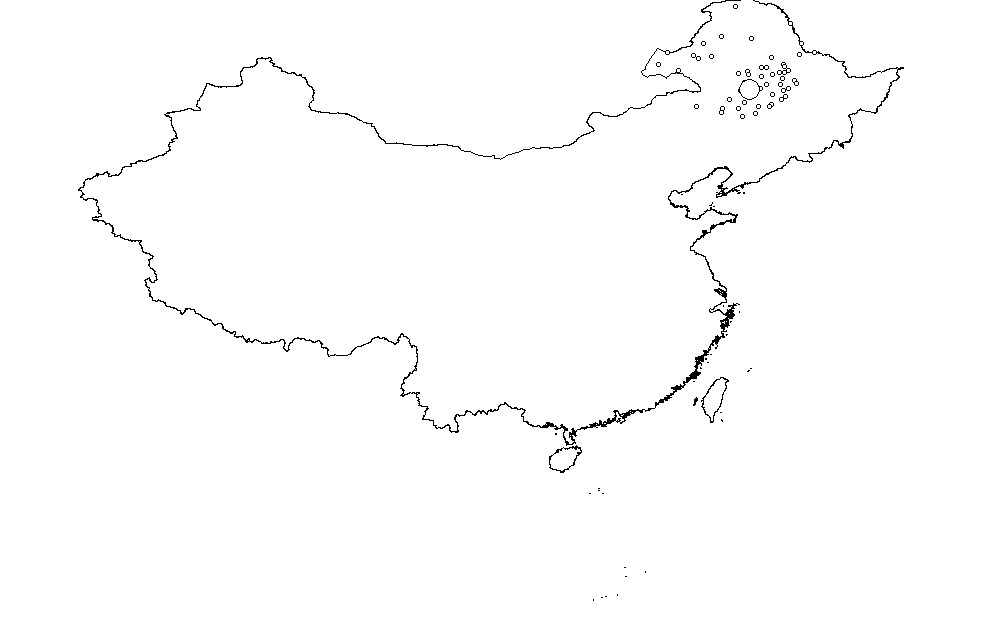
\includegraphics[angle=0,width=6cm]{pic//near.jpg}
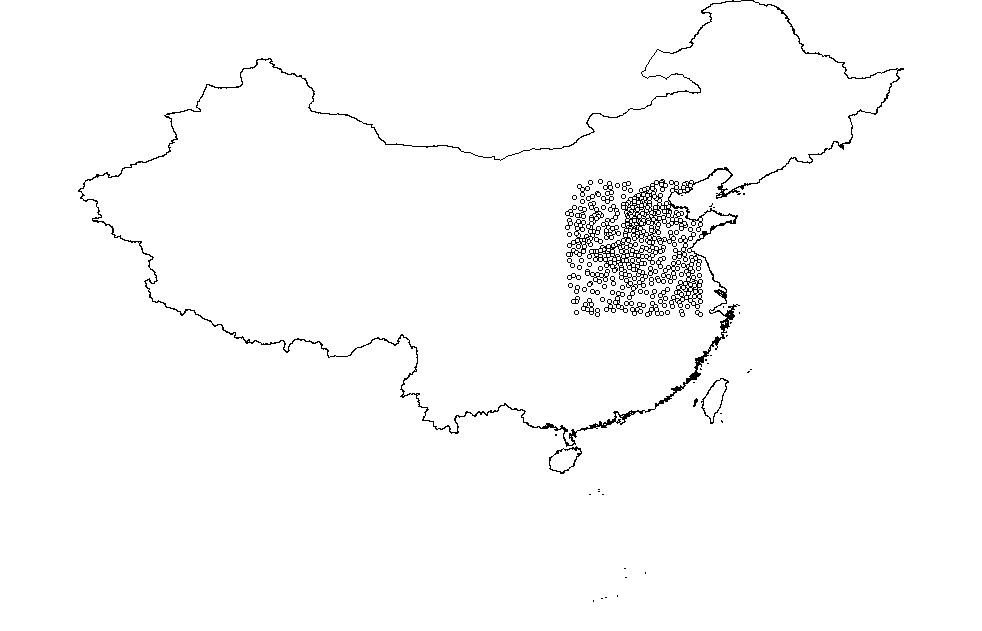
\includegraphics[angle=0,width=6cm]{pic//box.jpg}
\caption{临域查询与矩形范围查询结果}
\label{fig:9}
\end{center}
\end{figure}
%------
%------
\begin{figure}[h]
\begin{center}
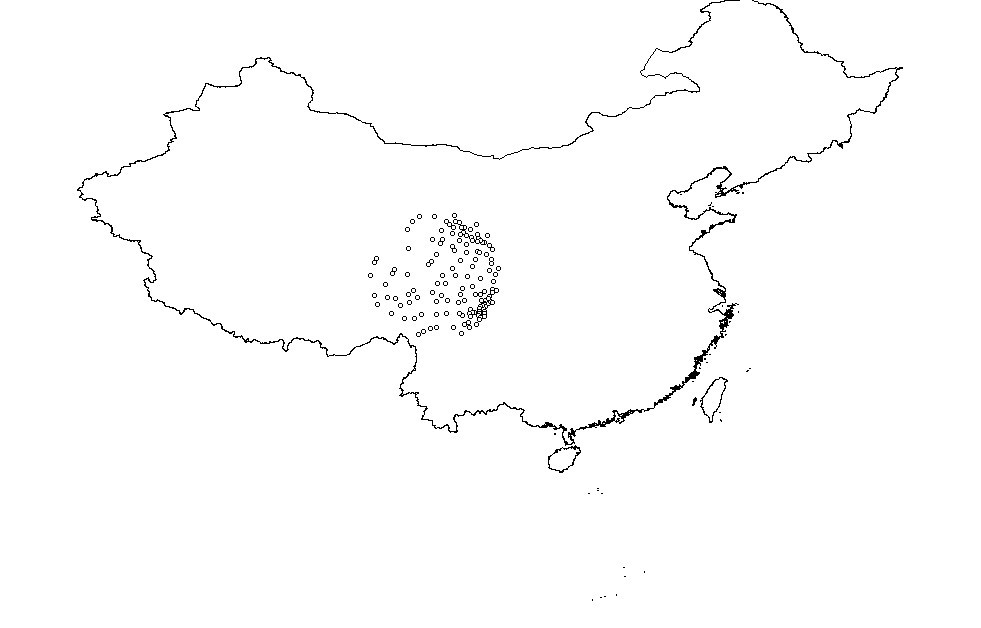
\includegraphics[angle=0,width=6cm]{pic//center.jpg}
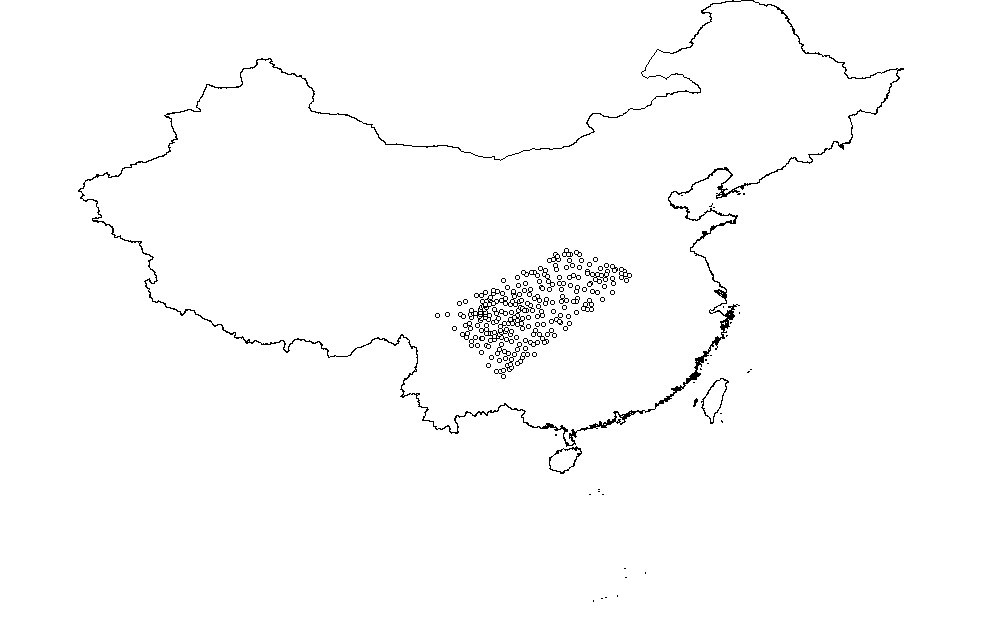
\includegraphics[angle=0,width=6cm]{pic//polygon.jpg}
\caption{圆形与多边形查询结果}
\label{fig:11}
\end{center}
\end{figure}
%------
MongoDB的范围查询操作支持的形状有矩形(\$box),圆形(\$center),多边形(\$polygon)。所查询的范围,默认是包含边界的。
 查询一个矩形范围,需要指定矩形的左下角和右上角两个坐标点,如下:

\noindent > box = [[80,40],[100,50]]\\
> db.xqpoint.find(\{''geom.coordinates'':\{\$within:\{\$box:box\}\}\})

查询结果如下图【】所示:

查询一个圆形范围,需要指定圆心坐标和半径,查询代码如下:

\noindent > center = [80,44]\\
> radius =5\\
> db.xqpoint.find(\{''geom.coordinates'':\{\$within:\{\$center:[center,radius]\}\}\})

查询结果如下图所示

    查询一个多边形范围,需要指定多边形的各个顶点,可以通过一个顶点数组或一系列点对象指定。其中,最后一个点是默认与第一个点连接的。如下:

\noindent > polygon1 = [[75,35],[80,35],[80,45],[60,40]]\\
> db.xqpoint.find(\{''geom.coordinates'':\{\$within:\{\$polygon:polygon1\}\}\})

查询结果如图所示

\subsection{总结}


\chapter{基于模型描述的数据抽取与推送}
\section{地学模型的参数化与描述}
现在的地学模型,主要是一些地学专业人员在同时具备地理学领域性专业知识和计算机有相当了解的基础上完成的。然而,实际任务中,操作人员往往不具备较深的地学专业知识,所以必须提供一套模型的高层描述方法,这就是任务模型描述法。任务模型描述方法是在任务和地学模型的认知基础上结合模型的数据数据的描述和输出表现形式,构建的 XML 语言描述。任务模型的用户主要有 3 种:1:应用领域人员,应用领域人员主要是最终用户,往往也是任务目标的制定者,他们对地学任务的掌握非常熟悉,但是计算机开发技术背景不足;2:地学模型的开发者,这类用户主要是构建者,对地学专业和计算机都有较深的了解;3:非人类用户,主要包括利用任务模型的软件或软件主体。但是由于缺乏对模型的统一的描述,和形式化的表达,是地学模型的应用存在多种问题:1:容易产生歧义,模型的数据输入的不明确,不能被计算机很好的理解,导致模型结果的偏差。2:可重用性低,模型建模过程中,通常设定在特定的任务环境中,并服务于特定的应用目标,很难为其他开发活动所利用。地学任务模型的描述需要满足三个条件:1:有效的获取和描述与应用领域相关的知识;2:能够满足不同用户的需求;3:要能够体现其重用性。本文采用面向数据的建模
方法,首先将模型划分为三个部分,通过对每个部分的具体描述,实现地学任务模型的结构化描述.

\subsection{模型的参数化及建立}
为了提高地学模型在各个层面的应用,提高地学模型的重用性,本文将地学模型划分为4个方面的内容:这里可以放一个图。
\begin{itemize}
\item 模型的主体层:
这部分主要是对模型的整体的认识,构建模型的主要要素,包括模型的条件,模型质量等的描述。
\item 模型的数据输入层:
这一层是模型的关键层,主要负责数据输入的对外接口部分,用于确认模型的数据需要的各种操作。
\item 模型的表现层:
这个部分主要是用于表现模型的最后运行结果输出方式和表现形式。
\item 模型的组件描述信息:
这部分是对模型运行过程中所涉及到的相关组件的属性信息的描述。
\end{itemize}

基于4层的模型描述体系,即模型主体-数据输入-模型表现-模型组件,下面对模型的各个部分分别做一个具体的介绍:
模型的主体层:这个部分描述了模型的应用,模型的构建目的,时间,名称, 分类标识信息, 适用范围,模型质量,模型性能,参数类型,运行条件,建模原理,求解方法集成模式,其他相关特征.
可用于对地理模型数据集的全面描述,数据集编目,及信息交换网络服务. 实施的对象可以是数据集,数据集系列,要素实体及属性.

\begin{table}[ht]
\caption{模型主体层} \label{table1}
\begin{center}
\begin{tabular}{lll}
\hline
 名称              &  定义                                            &  描述                                   \\
\hline
 模型的名字        &  模型的中文名字简称                              &  文本信息                               \\
 模型英文名字      &  模型的英文名字的简称                            &  文本                                   \\
 模型的内容信息    &  模型简介.开发目的                               &  文本                                   \\
                   &  进展情况                                        &                                         \\
 模型空间尺度      &  地理模型适用空间尺度                            &  空间信息                               \\
 模型时间尺度      &  地理模型适用时间尺度                            &  时间信息                               \\
 时间范围类型      &  说明模型模拟的时间范围                          &                                         \\
 模型的开发语言    &  模型开发中使用的语言                            &  采用的编程语言                         \\
 专题分类          &  对可用的地理模型进行分组                        &                                         \\
                   &  和查询所用的分类信息                            &                                         \\
 空间参考系统类型  &  \tabincell{c}{模型空间定位所用的参照系统\\类型}                     \\
 模型分类          &  \tabincell{c}{地理模型根据基内容.建模方法\\组织层次进行分类}        \\
 时空分类方法      &  依据模型同时间和空间关系进行分类                &  \tabincell{c}{ 动态模型,静态模型,\\连续模型,离散模型}   \\
 空间信息分类      &  \tabincell{c}{依据对空间信息的处理方式或包\\含空间异质性的程度}  &   \tabincell{c}{非空间模型,准空间模型,\\空间显式模型}    \\
 空间数据表达分类  &  依据对空间数据的表达进行分类                    &  栅格模型,矢量模型,混合模型           \\
\hline
\end{tabular}
\end{center}
\end{table}

模型的数据输入层:这个部分,主要是从模型的数据需求出发,强调对数据描述的统一性,无二义性,要保证数据的系统可识别性,所以从数据的类别,名称,格式,等信息进行描述。
\begin{table}[h]
\caption{模型的数据输入层} \label{table2}
\begin{center}
\begin{tabular}{lll}
\hline
 名字                   &  定义                               &  描述                       \\
\hline
 编码                   &  多源地学数据的分类编码             &  用于抽取时的数据类别识别   \\
 名称                   &  数据的名称                         &                             \\
 模型运行数据/过程数据  &  模型运行结果/模型运行产生的中间数  &  用于匹配数据抽取操作接口   \\
 运算分类               &  中间数据的运算方法                 &  用于匹配数据的操作接口     \\
 坐标(参照系统)       &  对空间数据的投影                   &  决定数据的投影转换函数     \\
 时间范围(开始,结束   &  决定要获取哪些年的数据             &  模型的运算年份             \\
 空间范围(extent)      &  决定要获取数据的范围               &  决定数据的剪切函数         \\
 基本单元(点,线面)   &  空间数据的类型                     &  决定采用的显示方式         \\
 变量交互格式           &  边界变量的数据交互格式             &  决定数据格式的转换方法     \\
 交互接口               &  用于边界变量交互的接口相关信息     &                             \\
\hline
\end{tabular}
\end{center}
\end{table}

模型的表现层是模型运行后产生的结果的可视化表示。主要是对输出数据格式,可视化形式的描写,具体内容如下表所示:

\begin{table}[ht]
\caption{模型的数据输入层} \label{table2}
\begin{center}
\begin{tabular}{lll}
\hline
 名字        &  定义                  &  描述                                        \\
\hline
 数据格式    &  数据的具体表现形式    &  用于将输出数据转换为系统可识别的数据格式    \\
 可视化方式  &  模型的可视化表现形式  &  用于匹配可视化数据操作接口                  \\
\hline
\end{tabular}
\end{center}
\end{table}

\subsection{模型描述}
本文采用了任务模型的分层描述方法,在非形式化层次的基础上,构建形式化的模型描述。
非形式化的描述更直观的表现模型具有的各项属性,包括模型名称,模型功能,模型编码,模型分类,模型约束信息,模型各输入参数,模型的输出表达。非形式化并不是意味着完全的无格式化,其实其内部往往需要明晰的结构化描述形式。本文为了确定任务模型的各项属性的非形式化特征,设计了模型表,如表1所示:

\begin{table}[ht]
\caption{非形式化描述} \label{table4}
\begin{center}
\begin{tabular}{lllll}
\hline
 非结构化模型描述  &            &            &        &            \\
\hline
 模型名称          &            &  模型类型  &        &  模型编码  \\
 时间范围          &            &            &        &            \\
 空间范围          &            &            &        &            \\
\hline
 输入参数1         &  参数名称  &  参数类型  &  限制  &  描述      \\
 输入参数2         &  参数名称  &  参数类型  &  限制  &  描述      \\
\hline
 输出表现1         &            &            &        &            \\
\hline
\end{tabular}
\end{center}
\end{table}

XML语言具有结构简单,高度可自定义,良好的表达能力和可扩充性的优点。同时XML是一种良构的,可实现异构环境下信息的交互。因此,XML可以为描述地学模型的空间,多源,动态等特性提供了条件。
半结构化的描述不仅仅便于模型的高效识别,和获取,而且更方便模型应用人员,开发人员的进一步交流,同时也为任务模型的形式化表述打下了良好的基础。

\begin{lstlisting}[language=xml]
<model_metadata>
    <!-- basic information -->
    <model_name>"模型名字"</model_name>
    <model_code>"模型编码"</model_code>
    <model_type>"模型类别"</model_type>
    <model_time_span>"模型研究时域"</model_time_span>
    <model_range>"模型研究区域"</model_range>
    <!-- input data information -->
    <input_data_1>
        <!-- detail input data information -->
        <input_data_name>"输入参数名1"</input_data_name>
        <input_data_type>"输入参数编码"</input_data_type>
        <input_data_limit>"输入参数限制"</input_data_limit>
        <input_data_discribe>"输入参数描述"</input_data_discribe>
    </input_data_1>
    <input_data_2>
        <!-- detail input data information -->
        <input_data_name>"输入参数名2"</input_data_name>
        <input_data_type>"输入参数类型"</input_data_type>
        <input_data_limit>"输入参数限制"</input_data_limit>
        <input_data_attributes>"输入参数属性"</input_data_attributes>
        <input_data_discribe>"输入参数描述"</input_data_discribe>
    </input_data_2>
    <!-- output expression -->
    <output_express>
        <!-- output detail -->
        <output_spatial_express>"输出空间表现"
		</output_spatial_express>
        <output_static_express>"输出统计表现"</output_static_express>
    </output_express>
</model_metadata>
\end{lstlisting}

\section{数据操作库的分类与描述}
数据操作库是架构在模型与数据库之间的桥梁,是转换数据库数据的方法集合,也是连接模型接口的适配器。对模型的数据 输入接口进行匹配,对模型输出接口进行识别,将模型的数据需求转换为对数据库数据的获取,基本运算和格式转换。

\subsection{数据操作的分类}
为了更好的区分数据操作库,基于模型对数据的具体需求,将数据操作库划分为以下四类:1格式转换库,2基本运算库,3数据抽取库,4可视化操作库。

1格式转换库:主要是针对模型的数据格式需求与数据库数据格式之间的不匹配问题,通常表现 为:
\begin{itemize}
\item 栅格数据
栅格数据有的需要按波段排列的数据 ,有的则需要按行或者按列存储的格式等等。本文的栅格数据按二进制流的方法存储在数据库中,针对模型 的不同需求,通过格式转换操作,将数据转换成对应的格式。
\item 矢量空间数据
空间数据格式是空间数据的基础,定义了如何在计算机中表达空间数据。各个GIS软件都定义了自己的空间数据格式。OGC定义了空间数据的交换格式,来实现各类GIS软件之间的空间数据交互。主要有WKT、WKB、GML几类。
\item 统计数据
统计数据的数据格式主要为dict字典类型,list列表类型,string字符串类型,vector数据类型等。

\end{itemize}

2基本运算库
基本运算库是数据转换中最主要的部分,实现数据

3:数据抽取
主要分为空间数据的抽取,栅格数据的抽取和统计数据的抽取

4可视化操作
主要是对空间分层的显示,统计分析的饼状图,线状图等的表现。


\subsection{数据操作的描述}
操作作为模型与数据之间的装置,规则化,结构化的操作描述,有利于模型与操作、操作与操作、操作与数据库之间的接口匹配,保证数据流的传递。

本文以XML作为结构化描述语言,对操作进行描述,将操作分为基本信息描述部分,数据输入部分,数据输出部分。
\begin{center}
\begin{lstlisting}[language=xml]

<basic information>
	<name>
	<function>
	<ID>
<input>
	<data type>
	<data code>
	<data classify>
<output>
	<data type>
	....
<>

\end{lstlisting}
\end{center}


\section{基于模型描述驱动的数据抽取}


\section{基于模型描述驱动的数据推送}







\end{document}
